\documentclass[12pt]{article}

\usepackage{fancyhdr}                       % Package: Fancy HDR
\usepackage{graphicx}
\usepackage[ngerman]{babel}
\usepackage{url}
\graphicspath{ {./images/} }

\title{Projektdokumentation: Frequenz-Analyse und Hall}        % Titel
\author{David Yaman [2321570], Dennis Räk [2385799]}            % Author
\date{HAW HAMBURG -- IT-Systeme -- SS 2021}                    % Datum/Kurs


\pagestyle{fancy}                           % eigener Seitenstil
\fancyhf{}                                  % alle Kopf- und Fußzeilenfelder bereinigen
\fancyhead[L]{ITS SS 2021}                  % Header links
\fancyhead[C]{}                             % Header Mitte
\fancyhead[R]{David Yaman [2321570], Dennis Räk [2385799]}      % Header rechts
\renewcommand{\headrulewidth}{0.4pt}        % Trennlinie (Oben)
\fancyfoot[C]{\thepage}                     % Seitennummer
\renewcommand{\footrulewidth}{0.4pt}        % Trennlinie (Unten)


\begin{document}
\maketitle
\newpage
\tableofcontents
\newpage
\section{Konzept}
Das entwickelte Gerät ist ein Hall-Effektgerät mit zusätzlicher Monitoring-Möglichkeit über Betrachtung des Frequenzspektrums des Ausgangssignals. 
Informationen über die Funktionsweise und Parameter werden über ein LCD-Display dargestellt und können mit Hilfe von vier Dreh-Encodern angepasst werden. 
Der Hall-Effekt hat die Parameter Room und Damping. Zusätzlich begrenzen Filtermodule das verhallte Signal im Frequenzbereich. 
Die variablen Grenzfrequenzen sind auch während der Darstellung des Frequenzspektrums veränderbar, um neben auditive auch visuelle Kontrolle zu ermöglichen. 
Der bandbegrenzte Hallanteil im Ausgangssignal lässt sich über Dry/Wet Kontrollieren. Zum gemeinsamen Arbeiten und festhalten der Arbeit wurde ein GitHub repository verwendet,
das unter folgender URL auffindbar ist:
\url{https://github.com/DennisR96/ITS_Gruppe03}
\section{Funktionen}
Die realisierten Funktionen umfassen einen Hall-Effekt, Low-/High-Cut und ein visualisiertes Frequenzspektrum des manipulierten Signals. 
Das Signal lässt sich über Cinch-Buchsen einspeisen und über Cinch-Buchsen oder Klinke wieder abnehmen.
Die Funktionen werden als einzelne Menüpunkte dargestellt und können mit Hilfe des Encoders A durchblättert werden. 
Encoder B, C und D steuern die Effekt- und Filterparameter, die per Knopfdruck auf ihren Ursprungswert zurücksetzbar sind.
\subsection{Hall-Effekt}
Der Hall-Effekt wird nach Start als Menüpunkt Eins angezeigt. 
Hier lassen sich die Parameter Room und Damping anpassen.
Zusätzlich kann der bandbegrenzte Hallanteil im Ausgangssignal mit Dry/Wet kontrolliert werden.
\subsection{Low-/High-Cut}
Low- und High-Cut sind im Routing hinter dem Hall-Effekt angesiedelt und werden im Menü als zweites dargestellt. 
Das verhallte Signal wird automatisch bandbegrenzt.  
Hier können die Grenzfrequenzen verschoben werden. 
Zudem lässt sich weiterhin der bandbegrenzte Hallanteil im Ausganssignal kontrollieren. 
\subsection{Frequenzspektrum (FFT)}
Menüpunkt Drei ist eine Darstellung des Ausgangssignals im Frequenzbereich. 
Der hörbare Frequenzbereich wird in 15 Balken aufgeteilt. Die Aufteilung orientiert sich an dem Hörverhalten des Menschen. 
Daher sind hohe Frequenzen breiter zusammengefasst als tiefe. 
Es können weiterhin dieselben Parameter wie in Menüpunkt Zwei angepasst werden.
\section{Umsetzung}
Die Umsetzung erfolgt mit Hilfe eines Teensy 4.1 Microcontrollers mit Audioboard, einem Display und vier Dreh-Encodern.
Für die Umsetzung wurden außerdem die Audio Library des Teensys, das GUI für Teensy Audioanwendungen, die Teensy optimierte ILI9341 Library und das Quadrature Phase Shift Encoding von John Main verwendet auf die später im Text näher eingegangen wird.
\\
\\
\begin{figure}[h]
  \centering
  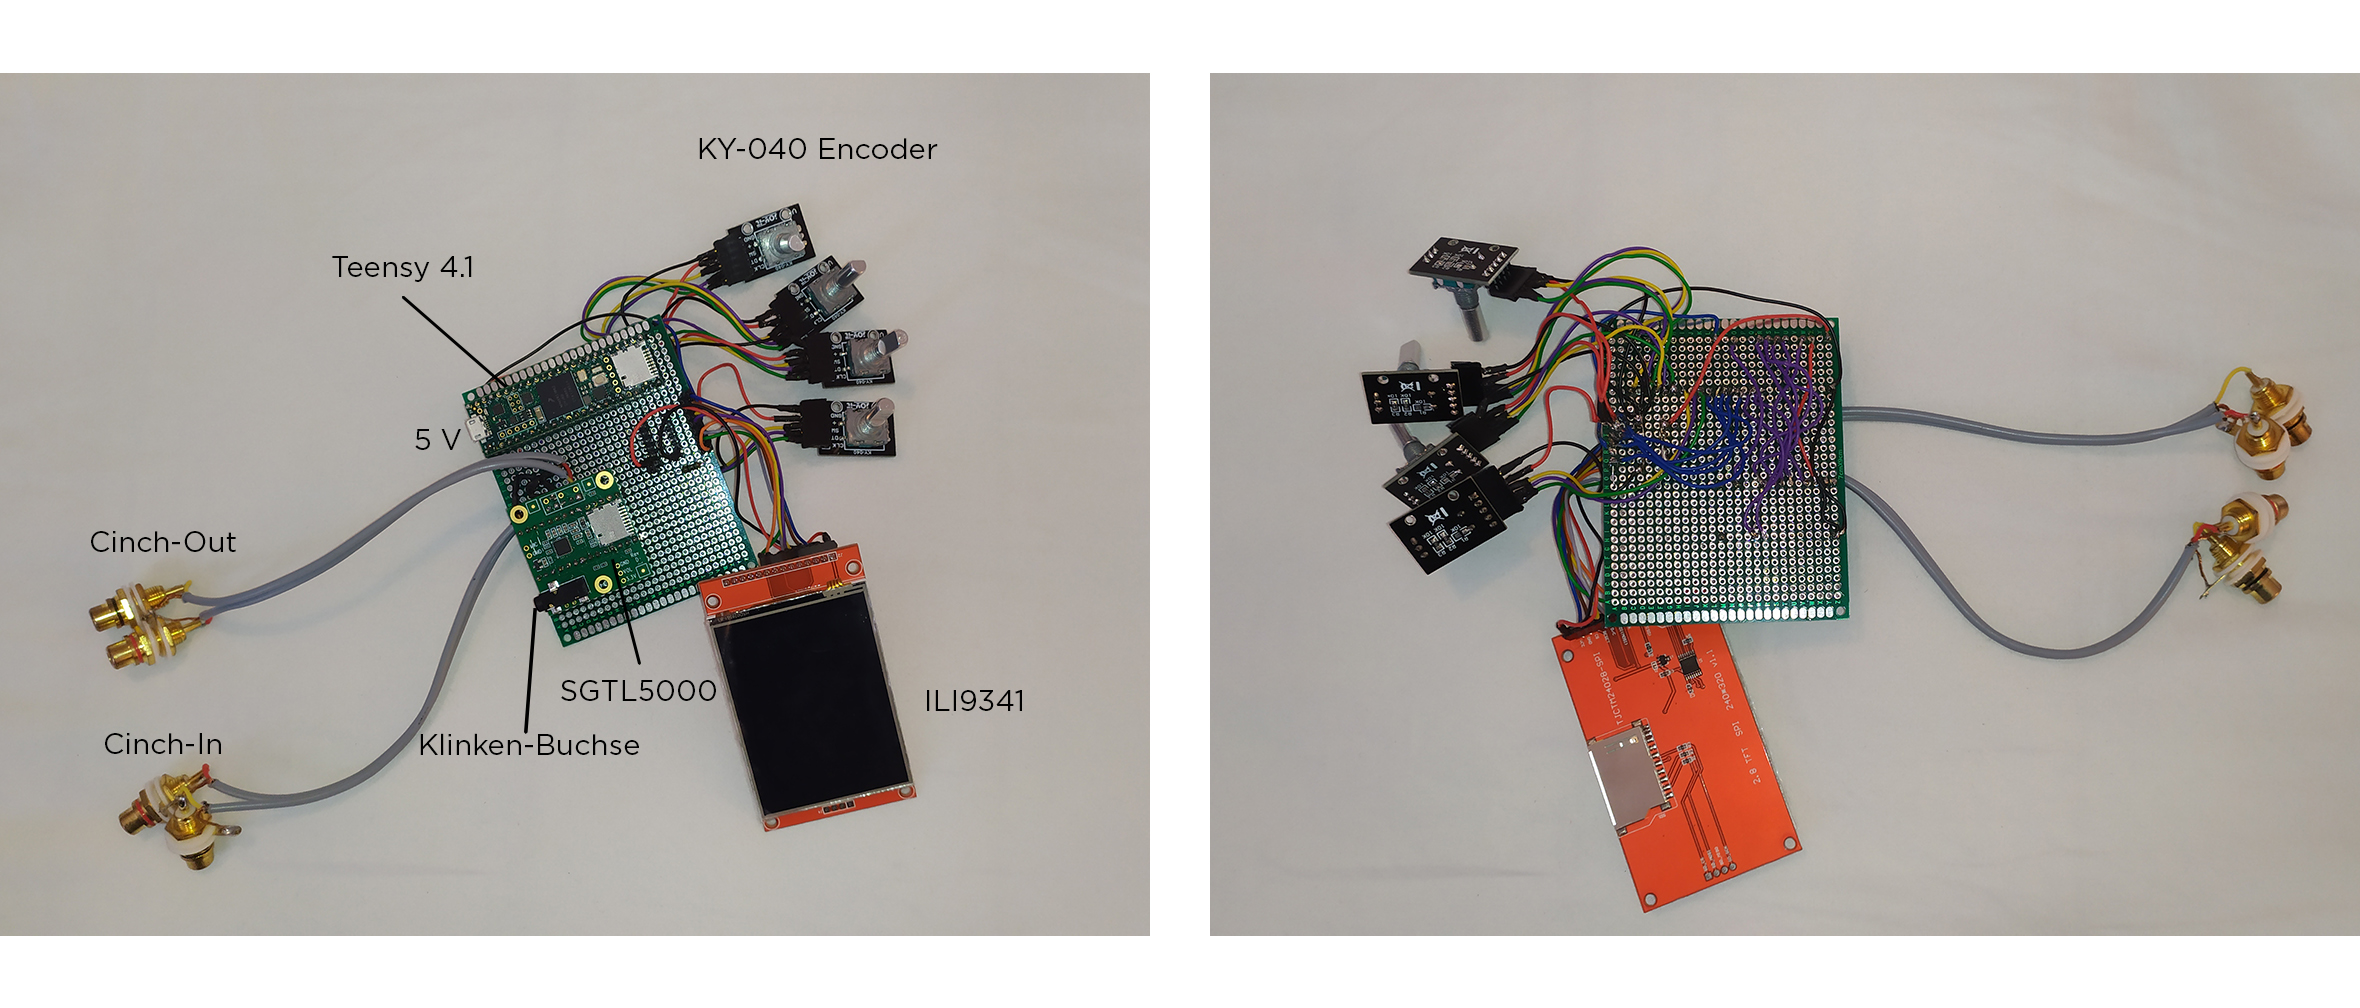
\includegraphics[width=\textwidth]{ITS_KomplettesGeraet.jpg}
  \caption{Vorderseite Gerät, Rückseite Gerät (v.l.n.r.)}
\end{figure}
\newpage
\subsection{GUI}
Das Userinterface ist in drei Menüpunkte aufgeteilt. Menüpunkt Eins gehört zum Hall-Effekt. Mittig wird auf dem Bildschirm \glq Reverb\grq{}\: angezeigt. 
Das untere Drittel des Displays ist in drei Kästen aufgeteilt die von links nach rechts Damping, Dry/Wet und Room und die jeweiligen Werte anzeigen. 
Damping und Room werden von 0 – 100, Dry/Wet von 0\% - 100\% angezeigt. Der Aufbau von Menüpunkt Zwei ist gleich, mittig wird \glq Filter\grq{}\: angezeigt. 
Die Parameter umfassen von links nach rechts Low-Cut, Dry/Wet und High-Cut. Low-Cut läuft zwischen 400 Hz und 12 kHz, High-Cut zwischen 12 kHz und 1,2 kHz, in einer Schrittweite von 100 Hz. 
Menüpunkt Drei zeigt die Frequenzanalyse an. Hier werden 15 Frequenzbänder mit ihrer momentanen Aussteuerung im Ausgangssignal in Form von Balken angezeigt. Balken Eins bis Vier stellen Frequenzen von 40 bis 860 Hz dar, Fünf bis Zehn Frequenzen von 860 bis 8,6 kHz und Elf bis Fünfzehn Frequenzen von 8,6 kHz bis 22 kHz.
Die Encoder sind gleich wie in Menüpunkt Zwei belegt.
Die Ansteuerung erfolgt über die Encoder nach folgendem Schema:
\begin{table}[h]
    \centering
    \caption{Encoder Belegung}
    \label{tbl:encoderbelegung}
    \begin{tabular}{l|l|l}
      \textbf{Encoder}  & \textbf{Funktion Hall} & \textbf{Funktion Filter/FFT}\\
      \hline
      A & Menü & Menü \\
   
      B & Damping & Low-Cut \\
   
      C & Dry/Wet & Dry/Wet \\
      
      D & Room & High-Cut \\
     

    \end{tabular}    

\end{table}
\\
\begin{figure}[h]
  \centering
  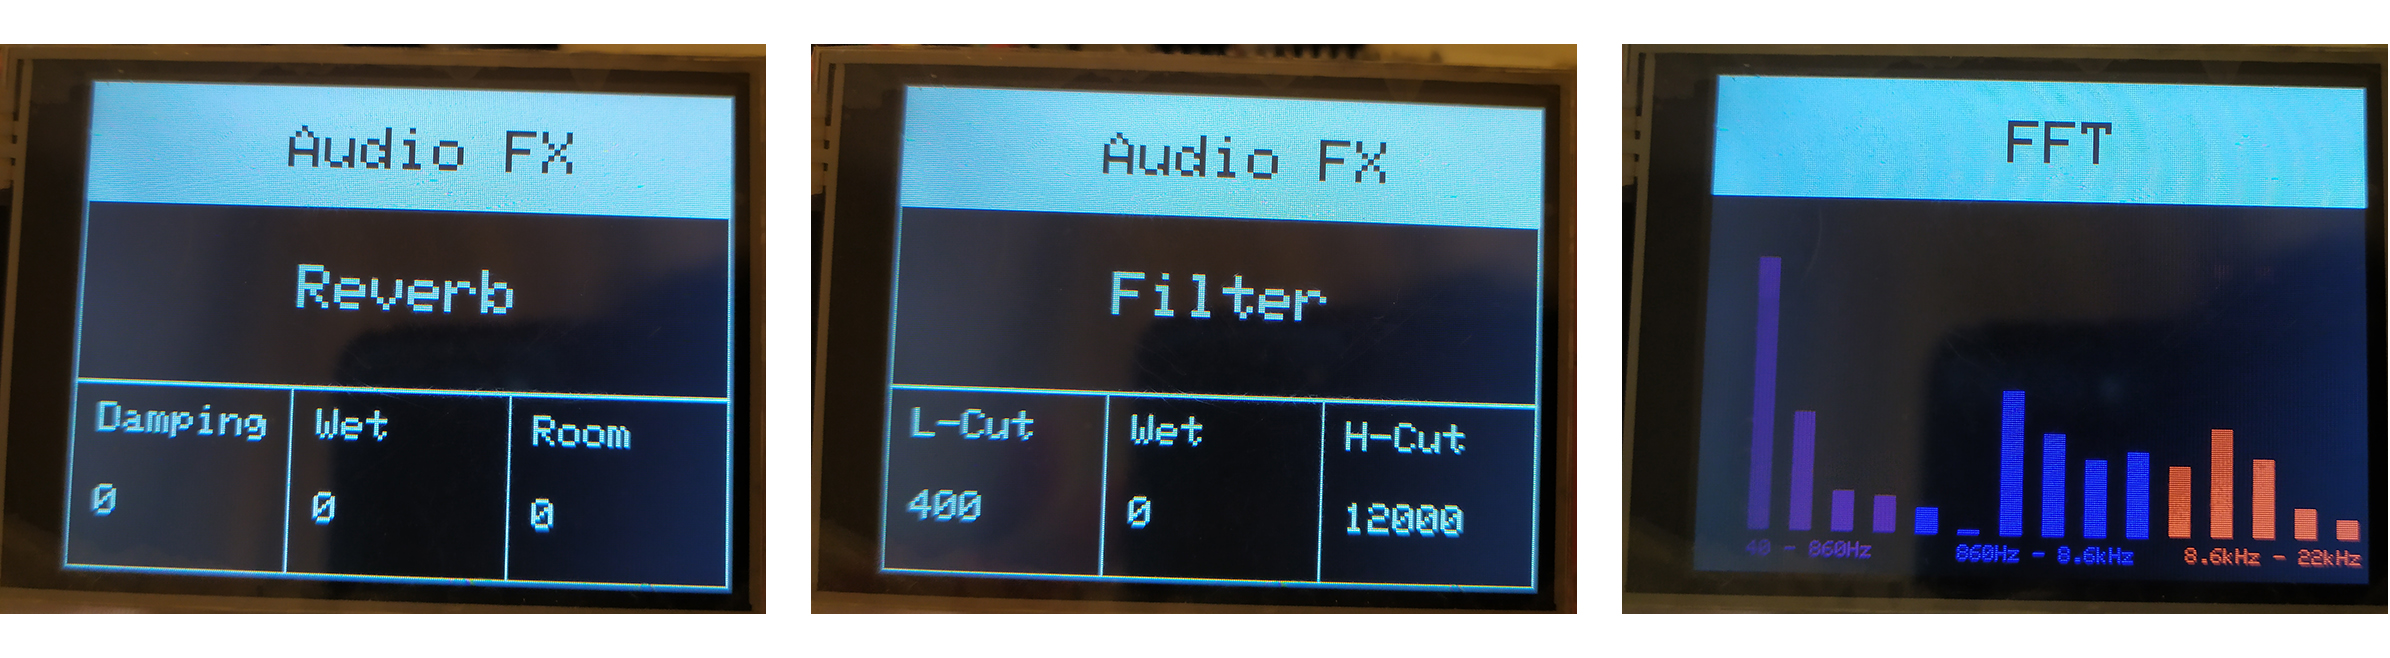
\includegraphics[width=\textwidth]{ITSMenue.jpg}
  \caption{Menüpunkt Eins bis Drei (v.l.n.r.)}
\end{figure}
\newpage

\subsection{Hardware und Schnittstellen}
Angeschlossen an den Teensy 4.1 ist das Teensy Audioboard SGTL5000 Rev D mit Cinch Ein- und Ausgängen, sowie einer Klinken-Buchse. 
Für die Anzeige des Menüs wird ein 2,8 Zoll TFT Display (ILI9341) 
genutzt und es werden vier KY-040 Dreh-Encoder der Marke Joy-It mit dem Micro-Controller verbunden. 
Für den Aufbau wird eine Lochrasterplatine verwendet. 

\subsubsection{SGTL5000 Audioboard}
Der SGTL5000 Audioboard ist mit dem Teensy 4.1 über möglichst kurze Kabelverbindungen verbunden. 
Die Abtastung erfolgt mit 44100 Samplewerten pro Sekunde und 16 Bit Quantisierungsstufen. 
Zur Ansteuerung des Chips wird das I2C Protokoll genutzt. 
Die Clockrates (LRCLK, BCLK \& MCLK) des Chips werden vom Teensy Microcontrollers vorgegeben. 
MCLK ist für die Synchronisation der internen Prozesse des AD-/DA-Wandlers verantwortlich.
Das Audiosignal wird über Cinch-Buchsen (Stereo) eingespeist und kann 
ebenfalls über Cinch-Buchsen (Stereo) oder eine Klinken-Buchse (Stereo) abgenommen werden.
In untenstehender Tabelle werden die Verbindungen zwischen Teensy 4.1 und Audioboard gezeigt.  
\paragraph{I2S}
Die diskreten Audiowerte werden mit dem Protokoll I2S übertragen und zurückgegeben. 
Im I2S Protokoll werden Channel L und Channel R über jeweils eine Multiplex-Verbindung gesendet oder empfangen. 
Die BCLK ist hierbei die wortlängenvorgebende Serial Clock und ein Produkt aus Samplerate, Bitrate und Channels. 
LRCLK gibt vor ob momentan rechter oder linker Channel übertragen werden. 
\paragraph{I2C}
Für die Kommunikation des Teensy 4.1 Mikrocontrollers mit dem Audio Adapter wird I2C genutzt. So wird der Chip kontrolliert und Parameter angepasst. 
Der Adapter befindet sich hierbei im \glq secondary mode\grq{}. Verbunden werden der Microcontroller und der Audio Adapter über SDA und SCL. 

\begin{table}[h]
  \centering
  \caption{Audioboard Verbindungen}
  \label{tbl:audioboardverbindungen}
  \begin{tabular}{l|l}
    \textbf{Audioboard Pin}  & \textbf{Teensy 4.1 Pins}\\
    \hline
    Audio Data & 7, 8, 20, 21, 23\\
 
    Audio Control	 & 18, 19\\
 
   

  \end{tabular}    

\end{table}

\subsubsection{ILI9341 TFT-Display}
Das verwendete Display umfasst 320x240px auf 2,8 Zoll in Farbe und wird mit 5 V versorgt.
Die Touch-Funktion wird in diesem Projekt nicht genutzt.
Angesteuert wird das Display über das SPI Bus-System.

\paragraph{SPI}
Das SPI Bus-System ermöglicht einen synchronen seriellen Datenbus. Hierbei ist das Display im \glq secondary mode\grq{}\:.
Über SCLK wird die Clockrate des Datenbuses definiert. Über \glq MOSI\grq{}\: können sukzessive Infowörter an das Display übermittelt werden, welches 
seinerseits über \glq MISO\grq{}\: simultan Infowörter an den Teensy zurückgibt. So können Grafik-Daten an das Display übergeben, aber auch Daten zur 
Fehlerreduktion und Spezifikationen wie z.B. die Displaygröße im Doppel-Duplex gesendet werden.
\\
\\
Die Verbindung von Teensy 4.1 und Display erfolgt nach untenstehender Tabelle:
\begin{table}[h]
  \centering
  \caption{Display Verbindungen}
  \label{tbl:displayverbindungen}
  \begin{tabular}{l|l}
    \textbf{Display Pin}  & \textbf{Teensy 4.1 Pins}\\
    \hline
    VCC & 5 V\\
 
    GND	 & GND\\
 
    CS	 & 10\\

    Reset	 & 3,3 V\\

    D/C	 & 9\\

    MOSI	 & 11\\

    SCK	 & 13\\

    LED	 & 5 V (mit 100 $\Omega$)\\

    MISO	 & 12\\
   

  \end{tabular}    

\end{table}
\subsubsection{KY-040 Encoder}
Die Encoder werden im Programmcode entprellt. Zusätzlich sind sie mit drei Vor-Widerständen von 10 k$\Omega$ vor den Datenleitungen beschaltet.
Durch gegenläufige Schalter-Verbindungen zwischen den Encoder-Anschlüssen kann erkannt werden, ob der Encoder sich im oder gegen den Uhrzeigersinn dreht.
Zudem kann über Knopfdruck der Zustand der Schalter-Verbindungen umgekehrt und somit als Impuls am Microcontroller wahrgenommen werden.
Durch die Funktionsweise sind die erzeugten Encoder-Daten im Gray-Mapping Schema. Dadurch wird eine höhere Fehlerresistenz erzielt.
Die Encoder werden mit 3,3 V versorgt.

\subsection{Programmcode}
Der Teensy 4.1 übernimmt mit seiner hohen Rechenleistung die Steuerung aller Funktionen. 
Das digitalgewandelte Audiosignal wird von ihm verhallt und bandbegrenzt. 
Währenddessen können Parameter und Grenzfrequenzen laufend verändert und über das Display ausgelesen werden. 
Auch die FFT wird vom Teensy durchgeführt und zur Visualisierung an das Display übergeben.
\subsubsection{main.cpp}
Die main ist das Herzstück des Programmcodes. Im Setup werden zuerst die Encoder initialisiert und anschließend das Display. 
Außerdem werden Audio-Board sowie zugehörige Effekte aktiviert. 
Durch die \glq encoder update\grq{}\:- Funktion wird innerhalb der Loop Funktion auf Änderungen im Status der Encoder gewartet.
\subsubsection{Control.h}
Mit der Bibliothek \glq Control.h\grq{} wird die allgemeine Ansteuerung initialisiert. 
Über Switch-Cases wird je nach Status des Encoders eine Menü-Variable und damit einer der drei Menüpunkte angewählt. Diese Information wird an \glq Display.h\grq{}\:übergeben 
und Parameterwerte der Effekte, sowie die Dry/Wet Zusammensetzung am virtuellen Audiomixer werden direkt angepasst.
\\
\\
\\
\\
\textbf{Beispiel:}
\\
Encoder A beeinflusst die Menü-Auswahl und steht auf dem Case 0. Wird nun der Encoder C gedreht, dann beeinflusst dieser die Dämpfung des Hall-Effektes.
Steht Enocder A auf dem Case 1, dann beeinflusst Encoder C die Grenzfrequenz des Low-Pass Filters.
\newpage
\subsubsection{Display.h}
Dieser Programmabschnitt enthält die Display Klasse. In dieser werden Funktionen bereitgestellt, um die Änderung an Encoder oder FFT bildlich darzustellen.  
Wechselt der Nutzer zu einem anderen Menüpunkt oder verändert einen Parameter, dann wird der jeweilige Bildschirmbereich zurückgesetzt und durch den aktuellen ersetzt. 
Nach diesem Muster funktionieren Menüpunkte, Parameter sowie FFT. Beim Start des Programmes wird ein kleines Intro geladen.
Wird Menüpunkt Drei aufgerufen, startet die FFT mit 1024 Samplewerten pro Sekunde. Somit erzeugt die FFT 511 Frequenzbänder die den jeweiligen Frequenzanteil (0 – 1) enthalten. 
Die Werte werden normiert und begrenzt auf die 15 Balken aufgeteilt und vom Display angezeigt. 
Die Milliseconds-Funktion steuert den Aktualisierungsintervall.  
Das Display-Layout wurde mit Hilfe der Adafruit ILI9341 Library in der Teensy optimierten Version von Paul Stoffregen erstellt.$^{[1]}$
\subsubsection{Encoding.h}
Die Encoding Bibliothek ist einer der wichtigsten Teile des Codes, da eine Bedienung ohne funktionierende Encoder nicht möglich ist. Um akkurate Veränderung am Encoder wahrzunehmen, 
müssen diese Entprellt werden. Bei der Wahl einer geeigneten Entprellung zeigte das Quadrature Phase Shift Encoding$^{[2]}$ von John Main gute Ergebnisse. Mit hoher Genauigkeit lassen sich 
kleine Veränderung am Encoder als +1 oder -1 wahrnehmen. Über die im Loop eingebettete encoder update Funktion wird eine Änderung am Encoder erkannt und in Form einer In- oder Decrementation an die Control 
Bibliothek weitergegeben. Die Knöpfe der Encoder werden durch die Bounce Library entprellt und ebenfalls über die Update Funktion überwacht.   
\newpage
\subsubsection{Shield.h}
Dieser Teil des Codes ist mithilfe des Teensy Audio System Design Tools generiert.$^{[3]}$ Hier wird das Routing des Eingangssignals durch die verschiedenen Effekte festgelegt. 
Die FFT-Funktion, der Hall-Effekt und die Filter wurden aus der Teensy Audio Library entnommen.$^{[4]}$
Aus einem Screenshot des Audio System Design Tools wird das im Code erzeugte Routing deutlich:
\\
\\
\\
\\
\begin{figure}[h]
  \centering
  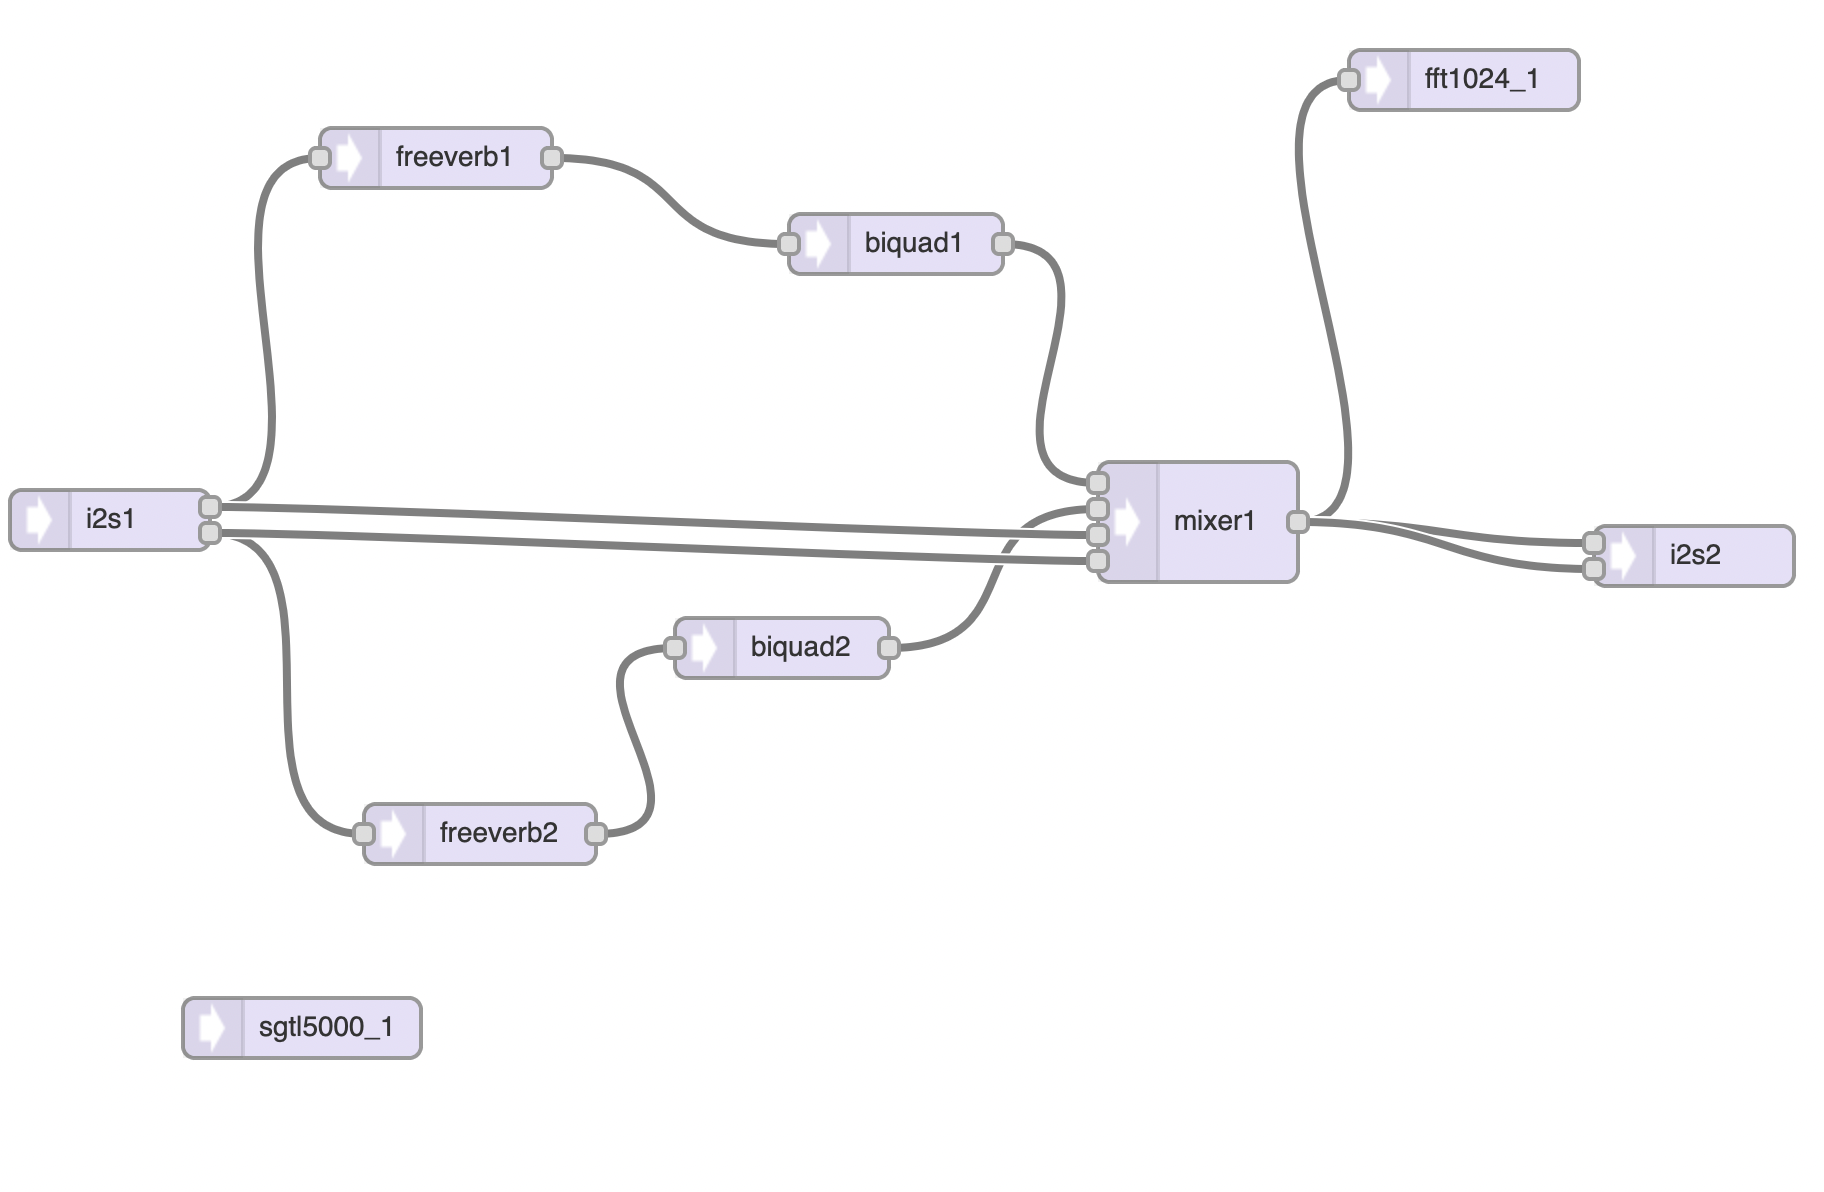
\includegraphics[width=\textwidth]{AudioDesignTool}
  \caption{Audio-Routing}
\end{figure}
\newpage
\section{Probleme}
In diesem Abschnitt werden die Hindernisse und Probleme bei der Realisation des Projektes beschreiben.
\subsection{Audio-Board}
Anfänglich kam es zu Schwierigkeiten beim Anschluss des Audio-Boards. Über normale Jumper Wire ist eine störfreie Signalwiedergabe nicht möglich. 
Erst durch Auflöten auf eine Lochrasterplattine ist eine Interferenzfreie Verbindung möglich und das Audio-Board funktioniert planmäßig.
\subsection{Einbinden von Effekten}
Im ursprünglichen Konzept sollte die eigenständige Programmierung von Audio-Effekten erfolgen. 
Dieses Verfahren ist an mehreren Stellen gescheitert. 
\\
\\
Viele Effekte lassen sich leicht in höheren Programmiersprachen
wie Python oder MATLAB realisieren, aber für eine effiziente Programmierung in Echtzeit werden viele erweiterte C Kenntnisse benötigt. 
Es ist zwar leicht das Konzept nachzubauen, aber ohne stabiles DSP Framework ist eine gute 
Performance nur schlecht möglich. 
\\
\\
Der Teensy erweist sich bei diesem Verfahren ebenfalls als eine Herausforderung. Bei Überwindung der ersten Herausforderung 
ist eine Einbindung in die bestehende Teensy Bibliothek notwendig. Dies ist sehr umständlich und ohne ein absolutes Verständnis nicht möglich. 
Leider gibt es von Seiten der Entwickler keine Anleitung eigene Effekte in die bestehende "Teensy Audio Library" einzubauen. 
\\
\\
Alles in allem führten diese Hindernisse zu einer Abkehr vom Bau eigener Effekte.  
\subsection{Verlust eines Teensy Boards}
Beim Anschluss der Drehencoder ist eine fehlerhafte Anbindung an die 5V Stromverbindung des Teensy entstanden. 
Da die Teensy PINs nicht 5V tolerant sind, führte dies zu einer Zerstörung eines Teensy Boards.
Für dieses musste ein Ersatzgerät erworben werden. 

  
\section{Fazit}
Trotz einiger Planänderungen ist das Projekt erfolgreich gewesen. Es ist ein funktionstüchtiger Hall-Effekt mit eingebauter Fast Fourier Transformation
entstanden.
Da einige Dinge wie das Einbinden von Effekten zum jetzigen Zeitpunkt noch nicht erreicht werden konnten, bietet das Projekt auch nach der IT-Systeme 
Veranstaltung Möglichkeiten der Weiterarbeit. Zur vorläufigen Vollendung des Projektes ist nun noch ein 3D gedrucktes Gehäuse geplant. 
Eventuell soll auch eine Akku-Stromversorgung mit Schiebeschalter integriert werden.
\newpage
\section{Quellen/Tools}
\lbrack1\rbrack\:\textbf{Paul Stoffregen}. (o. D.). Audio Adaptor Boards for Teensy 3.x and Teensy 4.x.
URL: 
\url{https://www.pjrc.com/store/teensy3_audio.html}
\\
\\
\textbf{Letzter Zugriff: 07.07.21}
\\
\\
\lbrack2\rbrack\:\textbf{Mikrocontroller.net: N/A}. (o. D.). I2S.
URL: 
\url{https://www.mikrocontroller.net/articles/I2S}
\\
\\
\textbf{Letzter Zugriff: 07.07.21}
\\
\\
\lbrack3\rbrack\:\textbf{Mikrocontroller.net: N/A}. (o. D.). I2C.
URL: 
\url{https://www.mikrocontroller.net/articles/I%C2%B2C}
\\
\\
\textbf{Letzter Zugriff: 07.07.21}
\\
\\
\lbrack4\rbrack\:\textbf{Mikrocontroller.net: N/A}. (o. D.). Serial Peripheral Interface.
URL: 
\url{https://www.mikrocontroller.net/articles/Serial_Peripheral_Interface}
\\
\\
\textbf{Letzter Zugriff: 07.07.21}
\\
\\
\lbrack5\rbrack\:\textbf{Mikrocontroller.net: N/A}. (o. D.). Drehgeber.
URL: 
\url{https://www.mikrocontroller.net/articles/Drehgeber}
\\
\\
\textbf{Letzter Zugriff: 07.07.21}
\\
\\
\lbrack6\rbrack\:\textbf{Paul Stoffregen und Limor Fried/Ladyada}. (2016). ILI9341\_t3: Optimized ILI9341 TFT Library.
URL: 
\url{https://github.com/PaulStoffregen/ILI9341_t3}
\\
\\
\textbf{Letzter Zugriff: 06.07.21}
\\
\\
\lbrack7\rbrack\:\textbf{John Main}. (o. D.). Robust Rotary encoder reading.
URL: 
\url{https://www.best-microcontroller-projects.com/rotary-encoder.html}
\\
\\
\textbf{Letzter Zugriff: 07.07.21}
\\
\\
\lbrack8\rbrack\:\textbf{Paul Stoffregen, et al.}. (o. D.). Audio System Design Tool for Teensy Audio Library.
URL: 
\url{https://www.pjrc.com/teensy/gui/}
\\
\\
\textbf{Letzter Zugriff: 07.07.21}
\\
\\
\lbrack9\rbrack\:\textbf{Paul Stoffregen, et al.}. (2014).  Teensy Audio Library.
URL: 
\url{https://github.com/PaulStoffregen/Audio}
\\
\\
\textbf{Letzter Zugriff: 07.07.21}
\end{document}
\end{justify}
